\subsection{Markov Decision Processes \label{MDP}}

A Markov Decision Process (MDP) is a model for an automatic 
decision making system. In the MDPTetris platform the agent
that plays the simulated games makes decisions modeled
after an MDP \citep{mdptetris}. The specifics of the 
MDPTetrsi platform is covered in section \ref{sec:MDPTetris}.
An MDP consists of a set of states $\MDPStates$,
a set of actions $\MDPActions$ and a 
\textit{state transition probability kernel} $\MDPTKernel$.
The states in $\MDPStates$ denotes all the states of the game
including the agent itself. In Tetris, the state is simply the
state of board in regards to which cells are
occupied by pieces and which are not. The state also contains
the current piece to be dropped by the controller.
The actions in $\MDPActions$
denotes all the actions that an agent may take. The $\MDPTKernel$ is
a probability function that determines how likely it is for an action 
to transition to another given state. As an example, given 3 states 
$\MDPState_0, \MDPState_1, \MDPState_2$, an action $\MDPAction_0$ and the 
agent currently being in state $\MDPState_0$. Then $\MDPTKernel$
might determine that taking action $\MDPAction_0$ transitions
to s $\MDPState_1$ with probability 0.2 and to state $\MDPState_2$
with probability 0.8. \\
The behaviour of the agent is defined by its policy $\policy$
which is a function that maps states of the game into actions, formally
defined as $\policy : \MDPStates \rightarrow \MDPActions$.
The goal is to find the best possible policy which in the case
of Tetris, is the policy that leads to the highest average score
in the game. The value of the policies are described as a 
\textit{value function} 
$\MDPValueFunction^{\policy}\left( \MDPState  \right)$ 
which maps a state
of the game into an expected value, namely the score of the 
agent when starting in the given state and follows
the policy $\policy$, formally defined as
$\MDPValueFunction^{\policy} : \MDPStates \rightarrow \mathbb{R}$. 
The optimal value function, that plays the game as well
as possible is denoted $\MDPValueFunction^{*}$. Optimizing the 
agent is a task that consists of determining a policy $\policy$ for which
$\MDPValueFunction^{\policy}$ gets as close to $\MDPValueFunction^{*}$
as possible. Finding the best policy for Tetris is a very computationally heavy 
task due to the enormous state space. Also, in the MDPTetris platform,
the agent will not be aware of the entire game state exactly to its 
size, but is rather use policies that are concerned with simplified
features of the game (described in detail in later sections). 
The methods in reinforcement learning provides various ways to
search for good policies.
One approach is 
Dynamic Programming (DP). The idea behind DP is to, for each state,
estimate the reward gained by the agent in for each possible action.
Yet, the DP approach is in the case of Tetris infeasible as it 
is a far too overwhelming task to comprehensively compute
the full traversal of the games state space. 
To give an intuition of this, consider
an MDP illustrated in figure figure \ref{fig:hypotheticalMDPGame}.
The MDP models a hypothetical game with a set of sates 
$\MDPStates = \{\MDPState_0, \MDPState_1, \MDPState_2, \MDPState_3,
\MDPState_4\}$ where the agent is given a reward of $\MDPReward_n$
for spending a time step in state $\MDPState_n$. The agent has a 
set of actions $\MDPActions = \{\MDPAction_0, \MDPAction_1, 
\MDPAction_2, \MDPAction_3, \MDPAction_4, 
\MDPAction_5, \MDPAction_6\}$ which causes the agent to transition 
between states in the game. In the figure, each circle/node illustrates a 
state, and the arrows shows the possible transitions between states.
Next to the arrow the action that causes the transition is listed 
along with the probability that if the action is committed, the particular 
transition takes place. For example, if the agent is in state $\MDPState_0$
and takes action $\MDPAction_0$, it will with probability 0.8 end
up in state $\MDPAction_0$ again and receive a reward of $\MDPReward_0$.
In this case, it is viable to compute the optimal policy by traversing
all states and compute the expected reward based on chosen actions.
Thus, for a policy $\policy$ DP allows one to obtain exactly the expected 
reward given to the agent when following $\policy$.
\begin{figure}[H]
\centering
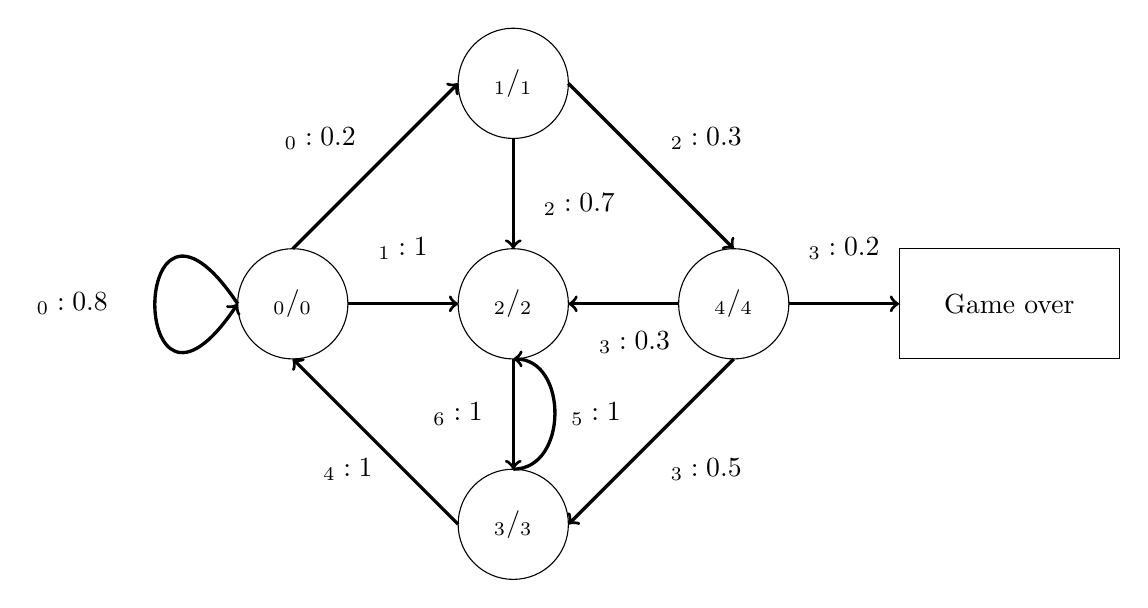
\begin{tikzpicture}[scale=0.7]
\draw  (0,0) ellipse (1 and 1);
\draw  (4,0) ellipse (1 and 1);

\draw  (4,4) ellipse (1 and 1);
\draw  (4,-4) ellipse (1 and 1);

\draw  (8,0) ellipse (1 and 1);

\draw [->, very thick](0,1) -- (3,4);
\draw [->, very thick](1,0) -- (3,0);
\draw [->, very thick](4,3) -- (4,1);
\draw [->, very thick](5,4) -- (8,1);
\draw [->, very thick](4,-1) -- (4,-3);
\draw [->, very thick](3,-4) -- (0,-1);
\draw [->, very thick](7,0) -- (5,0);
\draw [->, very thick](8,-1) -- (5,-4);
\draw [->, very thick](9,0) -- (11,0);

\node at (0,0) {$\MDPState_0 / \MDPReward_0$};
\node at (4,4) {$\MDPState_1 / \MDPReward_1$};
\node at (4,0) {$\MDPState_2 / \MDPReward_2$};
\node at (4,-4) {$\MDPState_3 / \MDPReward_3$};
\node at (8,0) {$\MDPState_4 / \MDPReward_4$};

\node at (0.5,3) {$\MDPAction_0: 0.2$};
\node at (-4,0) {$\MDPAction_0: 0.8$};
\node at (2,1) {$\MDPAction_1: 1$};
\node at (5.2,1.8) {$\MDPAction_2: 0.7$};
\node at (7.5,3) {$\MDPAction_2: 0.3$};
\node at (7.5,-3) {$\MDPAction_3: 0.5$};
\node at (6.2,-0.7) {$\MDPAction_3: 0.3$};
\node at (10,1) {$\MDPAction_3: 0.2$};
\node at (1,-3) {$\MDPAction_4: 1$};
\node at (5.5,-2) {$\MDPAction_5: 1$};
\node at (3,-2) {$\MDPAction_6: 1$};


\draw [->, very thick](4,-3) .. controls (5,-3) and (5,-1) .. (4,-1);
\draw [->, very thick](-1,0) .. controls (-3,3) and (-3,-3) .. (-1,0);

\draw [] (11,1) rectangle (15,-1);
\node at (13,0) {Game over};
\end{tikzpicture}
\caption{Example of a game formulated as an MDP \label{fig:hypotheticalMDPGame}}
\end{figure}

Tetris can be formulated very well as an MDP as well.
When looking at Tetris as an MDP, the state consists
of the current board configuration and the currently falling piece.
Figure \ref{fig:TetrisAsMDP} shows a visual presentation 
of how the game state is formulated into an MDP state. The black
blocks in the bottom of the board notes that these blocks are 
occupied and the text 'I-block' indicates that the currently
falling piece is an I-block.
The actions of the decision maker are hence partially deterministic.
The agent/controller can fully decide where the piece falls. However,
part of the state is the next pieces to be dropped, which is
randomly chosen from some distribution. The reward given to the agent
is based on how many lines it clears. If the agent appears in a state 
where it clears lines, the reward is exactly how many lines are cleared.
The reward is 0 in all other cases except for a state that ends the game.
The game over state typically leads to a massively negative reward to 
encourage the agent to play for as long as possible.
To get an intuition on why the exhaustive search through the Tetris 
state space is not an option, consider how Tetris is formulated as an MDP.
The state of the game is the configuration of the board combined with 
the current pieces to be dropped. Figure \ref{fig:TetrisAsMDP} shows
how the current board of the game can be considered as an MDP state. 
In this case, I-piece can be oriented either vertical or horizontal. 
In horizontal orientation, it can be dropped in 7 different columns,
and in vertical orientation it can be dropped in all 10 different columns.
When the piece is dropped, the next state of the game is the one 
where the I-piece occupies some space on the board, and the new falling piece
is one of the possible 7 pieces (see figure \ref{fig:TetrisPieces}) 
from the game which is chosen randomly 
out of the agents control. The state shown in figure \ref{fig:TetrisAsMDP}
thus have $17 \cdot 7 = 119$ transitions to other distinct states.
As all states have approximately the same number of transitions
and that the number of distinct states is enormous, the intuition 
clearly is that this cannot be exhaustive be computed with the Dynamic 
Programming approach.
\begin{figure}[H]
\begin{center}
\begin{tabular}{c c c c}
\textbf{Game board} & $\rightarrow$ & \multicolumn{1}{r}{\textbf{MDP state}}\\
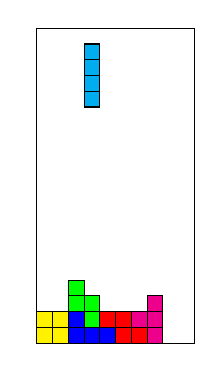
\begin{tikzpicture}[scale=0.2]
\draw [fill, yellow]  (0,2) node (v2) {} rectangle (2,0);
\draw [fill, blue] (2,2) rectangle (3,0);
\draw [fill, blue] (3,1) rectangle (5,0);
\draw [fill, red] (4,2) rectangle (6,1);
\draw  [fill,red](7,0) rectangle (5,1);
\draw [fill, green] (3,3) rectangle (4,1);
\draw [fill, green] (3,2) rectangle (2,4) node (v3) {};
\draw [fill, magenta] (7,3) node (v4) {} rectangle (8,0);
\draw [fill,magenta] (6,2) rectangle (7,1);
\draw [fill, cyan]  (3,19) node (v1) {} rectangle (4,15);
\draw  (v1) rectangle (4,18);
\draw  (4,17) rectangle (3,18);
\draw  (4,16) rectangle (3,17);
\draw  (3,16) rectangle (4,15);
\draw  (0,1) rectangle (8,0);
\draw  (v2) rectangle (8,1);
\draw  (2,3) rectangle (4,2);
\draw  (v3) rectangle (3,3) node (v5) {};
\draw  (v4) rectangle (8,2);
\draw  (1,2) rectangle (2,0);
\draw  (v5) rectangle (4,0);
\draw  (5,2) rectangle (6,0);
\draw  (7,2) rectangle (7,0);
\draw  (0,0) rectangle (10,20);
\end{tikzpicture} & &
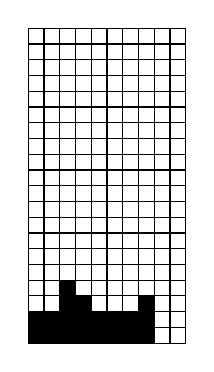
\begin{tikzpicture}[scale=0.2]
\draw [fill,black] (0,0) rectangle (8,2);
\draw [fill,black] (2,2) rectangle (3,4);
\draw [fill,black] (3,2) rectangle (4,3);
\draw [fill,black] (7, 2) rectangle (8,3);
\draw  (0,0) rectangle (10,20);
\draw  (1,20) rectangle (2,0);
\draw  (3,20) rectangle (4,0);
\draw  (5,20) rectangle (6,0);
\draw  (7,20) rectangle (8,0);
\draw  (9,20) rectangle (10,0);
\draw  (0,19) rectangle (10,18);
\draw  (0,17) rectangle (10,16);
\draw  (0,15) rectangle (10,14);
\draw  (0,13) rectangle (10,12);
\draw  (0,11) rectangle (10,10);
\draw  (0,9) rectangle (10,8);
\draw  (0,7) rectangle (10,6);
\draw  (0,5) rectangle (10,4);
\draw  (0,3) rectangle (10,2);
\draw  (8,1) rectangle (10,1);
\end{tikzpicture} & I-block
\end{tabular}
\end{center}
\caption{Illustration of how Tetris can be formulated as an MDP. 
\label{fig:TetrisAsMDP}}
\end{figure}

However, another and more viable solution is in this 
case the \textit{Monte Carlo} methods \citep{Csaba}. 
With the \textit{Monte Carlo} method, the goal is to learn
the value of $\MDPValueFunction^{\policy}$, in our case, 
we typically wish to estimate the value function from the starting 
state of the game. Using the method, the episode is simulated 
and the agent will interact with the environment with the given policy
and finally exit with an estimate of $\MDPValueFunction^{\policy}$,
in our case, the final score. Thus, using this method, we need not search 
through the entire state set, and neither do we need to know all
details of the game states the agent went through while playing.
Hence, the \textit{Monte Carlo} approach fits the case of Tetris
very well as we cannot afford to comprehensively  model the entire 
state space, but only need assess the performance of a policy from the 
starting state of the game.
How the feedback from the simulation is used to obtain better policies
is discussed in detail in the section 
\ref{Optimizers} on page \pageref{Optimizers}.










 


